\documentclass[UTF8]{ctexart} 

\usepackage{graphicx}
\usepackage{amsmath}
\usepackage{amssymb}
%v26.3.26
%test 26
\begin{document}

\begin{figure}[t]
  \centering
  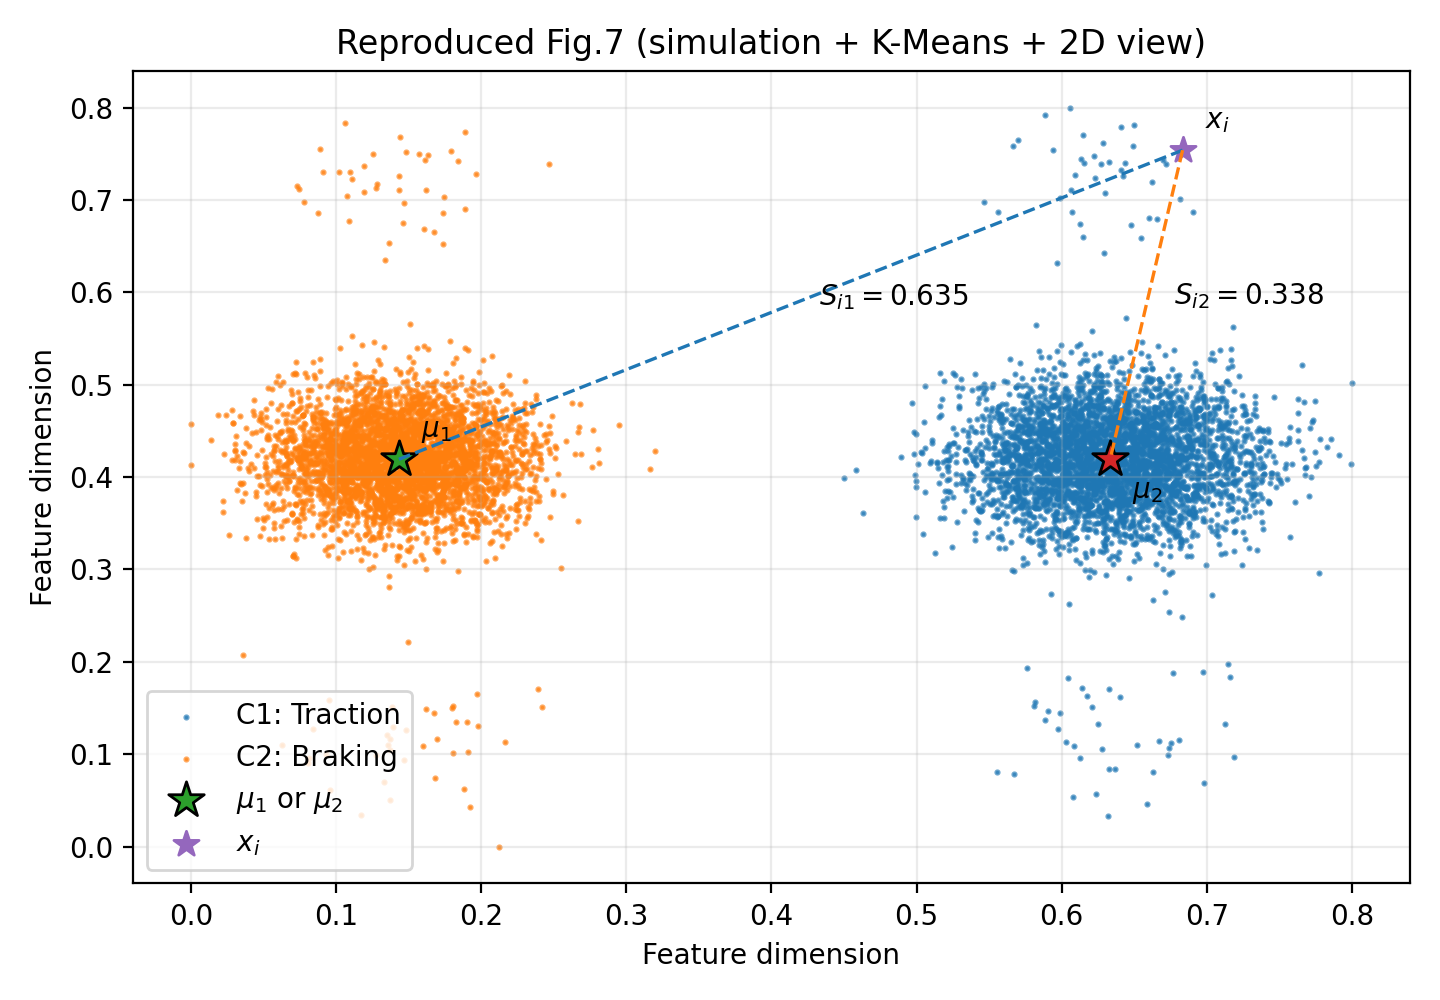
\includegraphics[width=0.9\linewidth]{fig71.png}
  \caption{Simulation + K-Means + PCA 2D view 的聚类可视化结果（fig71）。散点为样本在二维投影空间的坐标，颜色表示 K-Means 的簇标签；星号为簇中心；紫色星号为选取的样本点 $x_i$，虚线段及标注为其到两个簇中心的欧氏距离 $S_{i1},S_{i2}$。}
  \label{fig:fig71}
\end{figure}

\paragraph{图 \ref{fig:fig71} 的生成流程（对应当前代码逻辑）}
首先构造每个时刻的本地原始特征向量
\begin{equation}
  x_i=\bigl[U_{\mathrm{sub}}(i),\;\frac{\mathrm{d}U_{\mathrm{sub}}}{\mathrm{d}t}(i),\;I_{\mathrm{sub}}(i)\bigr]^\top\in\mathbb{R}^3,
\end{equation}
其中 $U_{\mathrm{sub}}$、$\mathrm{d}U_{\mathrm{sub}}/\mathrm{d}t$ 与 $I_{\mathrm{sub}}$ 由仿真随机生成（牵引/制动工况分段切换，并加入噪声）。对特征做标准化得到
\begin{equation}
  \tilde{x}_i=\frac{x_i-\mu_x}{\sigma_x},
\end{equation}
并在 $\{\tilde{x}_i\}$ 上执行 K-Means 聚类（$K=2$），得到簇标签 $c_i\in\{1,2\}$ 与簇中心
\begin{equation}
  \tilde{\mu}_k=\frac{1}{|\mathcal{C}_k|}\sum_{i\in\mathcal{C}_k}\tilde{x}_i,\quad k\in\{1,2\}.
\end{equation}

\paragraph{PCA 投影（用于二维可视化）}
由于原始特征为三维，图 \ref{fig:fig71} 仅用于可视化，因此将标准化后的点云通过 PCA 投影到二维。记样本协方差为
\begin{equation}
  \Sigma=\frac{1}{N}\sum_{i=1}^N(\tilde{x}_i-\bar{\tilde{x}})(\tilde{x}_i-\bar{\tilde{x}})^\top,
\end{equation}
取 $\Sigma$ 的前两大特征值对应的单位特征向量组成投影矩阵
\begin{equation}
  W_2=[w_1,w_2]\in\mathbb{R}^{3\times 2},
\end{equation}
则二维坐标（PCA 得分）为
\begin{equation}
  z_i=W_2^\top \tilde{x}_i\in\mathbb{R}^2,\qquad
  z_{\mu_k}=W_2^\top \tilde{\mu}_k\in\mathbb{R}^2.
\end{equation}
代码中进一步对 $\{z_i\}$ 与 $\{z_{\mu_k}\}$ 做 Min-Max 缩放到 $[0,0.8]$ 区间，以匹配图形展示尺度（因此坐标上限出现 $0.8$；该数值是显示尺度设定，并非物理量）。

\paragraph{距离标注}
在二维可视化空间中选取一个样本点 $x_i$（图中紫色星号），计算其到两个簇中心的欧氏距离并绘制虚线：
\begin{equation}
  S_{i1}=\lVert z_i-z_{\mu_1}\rVert_2,\qquad
  S_{i2}=\lVert z_i-z_{\mu_2}\rVert_2.
\end{equation}
需要强调的是，PCA 坐标是原特征的线性组合，主要用于展示聚类分布形态，本身不具备直接物理量含义。

\end{document}
